\documentclass[english,11pt]{article}

\pdfoutput=1

\usepackage[T1]{fontenc}
\usepackage[latin9]{inputenc}
\usepackage{verbatim}
\usepackage{float}
\usepackage{amsthm}
\usepackage{amsmath}
\usepackage{amssymb}
\usepackage{graphicx}
%\usepackage{multirow}
\usepackage{color}
\usepackage{url}
\usepackage{caption}
\usepackage{subcaption}
\usepackage{mathtools} 
\usepackage[margin=1.2in]{geometry}


\newcommand{\LL}{\mathcal{L}}
\newcommand{\E}{\mathbb{E}}
\newcommand{\I}{\mathcal{I}}
\newcommand{\ep}{\varepsilon}
\newcommand{\Z}{\mathbb{Z}}
\newcommand{\GCD}{\mathbf{GCD}}
\newcommand{\XX}{\mathcal{X}}
\newcommand{\SUM}{\text{sum}}
\newcommand{\1}{\mathbf{1}}


\newcommand{\TODO}[1]{{\color{red}{[#1]}}}

\makeatletter

%%%%%%%%%%%%%%%%%%%%%%%%%%%%%% Textclass specific LaTeX commands.
\numberwithin{equation}{section}
%\numberwithin{figure}{section}
\theoremstyle{plain}
\newtheorem{thm}{\protect\theoremname}[section]
\theoremstyle{definition}
\newtheorem{defn}[thm]{\protect\definitionname}
\theoremstyle{remark}
\newtheorem{claim}[thm]{\protect\claimname}
\theoremstyle{plain}
\newtheorem{lem}[thm]{\protect\lemmaname}

\newtheorem*{lem*}{Lemma}

\theoremstyle{remark}
\newtheorem{rem}[thm]{\protect\remarkname}
\theoremstyle{plain}
\newtheorem{corollary}[thm]{\protect\corollaryname}
\theoremstyle{plain}
\newtheorem{proposition}[thm]{\protect\propositionname}
%%%%%%%%%%%%%%%%%%%%%%%%%%%%%% User specified LaTeX commands.
%\usepackage{slashbox}

\usepackage{babel}
\providecommand{\claimname}{Claim}
\providecommand{\definitionname}{Definition}
\providecommand{\lemmaname}{Lemma}
\providecommand{\remarkname}{Remark}
\providecommand{\theoremname}{Theorem}
\providecommand{\corollaryname}{Corollary}
\providecommand{\propositionname}{Proposition}


\newcommand{\reals}{\mathbb{R}}
\newcommand{\RL}{\mathbb{R}^L}
\newcommand{\CL}{\mathbb{C}^L}
\newcommand{\RN}{\mathbb{R}^N}
\newcommand{\RNN}{\mathbb{R}^{N\times N}}
\newcommand{\CNN}{\mathbb{C}^{N\times N}}
\newcommand{\inner}[1]{\left\langle {#1} \right\rangle}
\newcommand{\hx}{\hat{x}} 
\newcommand{\one}{\mathbf{1}} 
\newcommand{\SNR}{\ensuremath{\textsf{SNR}}}

\begin{document}

\title{Estimation below the detection limit with application to cryo-em}


\author{Tamir Bendory, Nicolas Boumal, William Leeb, Eitan Levin and Amit Singer}
\maketitle

\begin{abstract}
	Here comes the abstract
\end{abstract}

\section{Introduction}

We consider the problem of estimating a signal from its multiple occurrences in a measurement. In the high SNR regime, the problem is easy. In the low SNR, it becomes interesting and that is the focus of this paper. 
The problem can be posed as blind deconvolution between the signal and a sparse binary signal.
We can also consider the extension for multiple signals. 

The main motivation for this paper arises from single particle reconstruction using cryo-electron microscopy (cryo-EM). In cryo-EM, multiple samples .....  

in low SNR detection is impossible. This led to the belief in the cryo-EM community is reconstruction of small molecules is impossible. We claim that this argument is wrong. While this paper focused on the mathematical toy model, Section TKTK discusses the application to cryo-EM. A companion paper focused on this application and provides all the details~\cite{bendory2018toward}. 

\begin{figure}[t]
	\centering
	\begin{subfigure}[h]{0.33\textwidth}
		\centering
		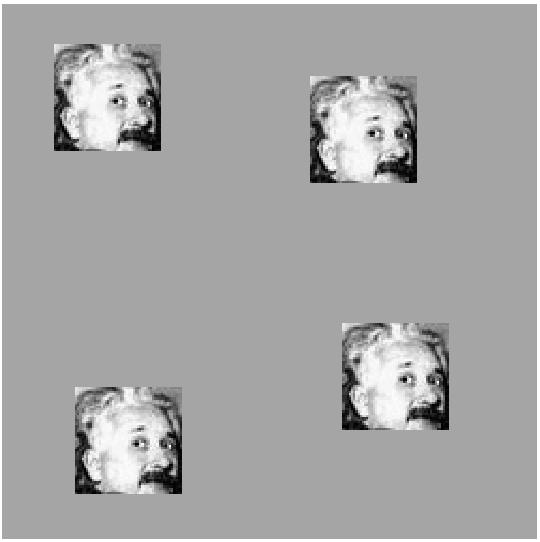
\includegraphics[scale=0.5]{micrograph_Einstein_example_clean}
		\caption{$\sigma = 0$}
	\end{subfigure}%
	\begin{subfigure}[h]{0.33\textwidth}
		\centering
		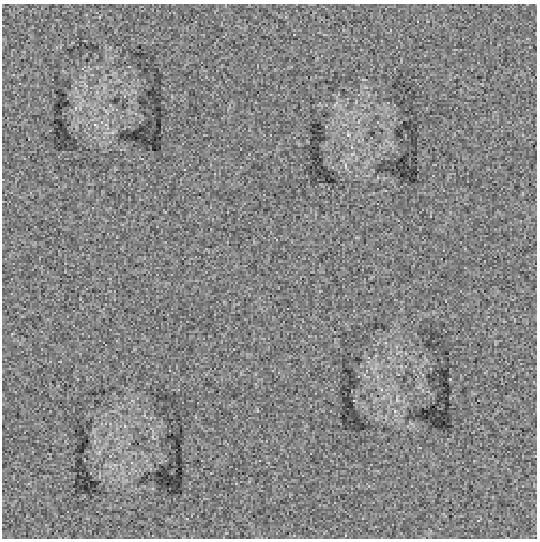
\includegraphics[scale=0.5]{micrograph_Einstein_example_s05}
		\caption{$\sigma = 0.5$}
	\end{subfigure}
	\begin{subfigure}[h]{0.33\textwidth}
		\centering
		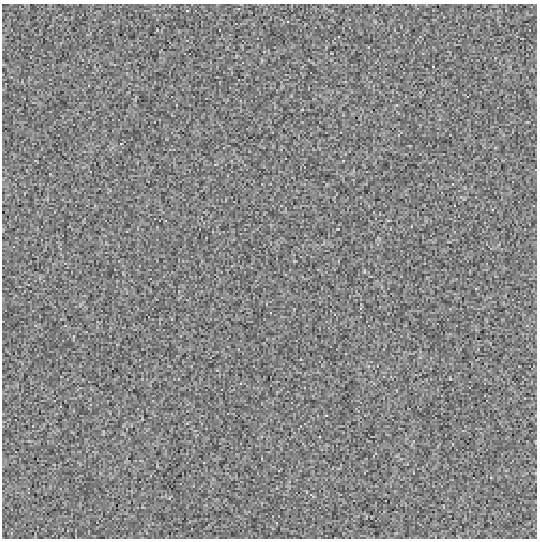
\includegraphics[scale=0.5]{micrograph_Einstein_example_s3}
		\caption{$\sigma = 3$}
	\end{subfigure}
	\caption{\label{fig:micro_example} Example of micrographs of size $250\times 250$ with additive white Gaussian noise of variance $\sigma^2$ for increasing values of $\sigma$. Each micrograph contains the same four occurrences of a $50 \times 50$ image of Einstein. In panel (c), the noise level is such that it is very challenging to locate the occurrences of the planted image. In fact, it can be shown that at low $\SNR$, reliable detection of individual image occurrences is impossible, even if the true image is known. By analogy to cryo-EM, this depicts a scenario where particle picking cannot be done.}	
\end{figure}

\subsection{Model}


Let $x_1,\ldots,x_K\in\RL$ be the sought signals and let $y\in\RN$ be the observed micrograph (notice that it is equivalent to think of the data as being one long micrograph or multiple shorter micrographs concatenated into one.)
The forward model (or ``image'' formation model) is as follows. For each target signal $x_k$, an unknown binary signal $s_k \in \{0, 1\}^{N-L+1}$ indicates (with 1's) the starting positions of all occurrences of $x_k$ in $y$, so that, with additive white Gaussian noise:
\begin{align}
y & = \sum_{k=1}^K x_k \ast s_k + \varepsilon, & \varepsilon & \sim \mathcal{N}(0,\sigma^2 I_N),
\label{eq:model}
\end{align}
where $\ast$ denotes linear convolution. The binary signals obey the following property:
\begin{align}
\textrm{If } s_k[i] = 1 \textrm{ and } s_{k'}[j] = 1 \textrm{ but } (k, i) \neq (k', j), \textrm{ then } |i - j| \geq 2L-1.
\label{eq:spacing}
\end{align}
In words: the starting positions of any two occurrences (be it of the same signal or of two different signals) must be separated by at least $2L-1$ positions, so that their end points are necessarily separated by at least $L-1$ signal-free entries in the micrograph.
It can be also extended to Poison model; see Section TKTK.


From $y$, we aim to recover $x_1, \ldots x_K$, and possibly also the number of occurrences of each. In contrast, particle picking is the task of estimating the binary signal $s = s_1 + \cdots + s_K$, while clustering is the task of separating $s$ into its components $s_1, \ldots, s_K$. Neither of the latter can be performed reliably if $\sigma$ is large (that is, at low $\SNR$.)

%We denote the set of these nonzero values by 
% $\mathcal{S}_i$ and its cardinality by $\vert \mathcal{S}_i\vert = M_i$. 
%By assuming that all $\mathcal{S}_i$'s are disjoint,  we let $s = \sum_{i=1}^Ks_i$, $\mathcal{S} = \bigcup_{i=1}^{K} \mathcal{S}_i$ and  $\vert \mathcal{S}\vert :=M =  \sum_{i=1}^{K}M_i$.  %Neither the $M_i$'s nor $M$ are assumed to be known.


Considering~\eqref{eq:model}, one can think of this inverse problem as a mixture of blind deconvolution problems between binary signals and the target signals. %Related literature is briefly surveyed in Appendix~\ref{sec:related_literature}.

We derive algebraic relations between the autocorrelation functions of the micrographs and the autocorrelation functions of the target signals. For ease of exposition, we do so in the 1-D case. Extension to the 2-D case is straightforward. We also give additional technical details regarding the two experiments presented in Section~\ref{sec:results}.



\subsection{Related work}

For $K=1$, our problem can be interpreted as a special case of the system identification problem. Similarly to~\eqref{eq:model}, the system identification forward model takes the form
%
\begin{math}
%
y = x\ast w + \varepsilon,  
%
\end{math} 
%
where $x$ is the unknown signal (the ``system''), $w$ is an unknown, random, input sequence, and $\varepsilon$ is an additive noise.   
%The problem has also been studied in the case of a known input $w$~\cite{pillonetto2010new,dinuzzo2015kernels,bottegal2016robust}. 
The goal of this problem is to estimate $x$, usually referred to as ``identifying the system.'' The question of identifiability of $x$ under this observation model is addressed for certain Gaussian and non-Gaussian $w$ in~\cite{benveniste1980robust,kormylo1983identifiability}. In the special case where $w\in\{0,1\}^N$, satisfying the spacing requirement~\eqref{eq:spacing}, we obtain our model in the  case of a single signal ($K = 1$). The same observation model is used for blind deconvolution, a longstanding problem arising in a variety of engineering and scientific applications such as astronomy, communication, image deblurring, system identification and optics; see~\cite{jefferies1993restoration,shalvi1990new,ayers1988iterative,abed1997blind}, just to name a few. 
%\TODO{ref this by Giannakis: \cite{giannakis1989identification}}

%%%To make the problem well-posed, we must  assume some prior knowledge or  structure.  In our case, the prior information is that $s$ is a binary signal that satisfies the separation constraint~\eqref{eq:spacing}.  Other settings of blind deconvolution problems have been analyzed recently, see for instance~\cite{ahmed2014blind,li2016identifiability,li2016rapid,ling2015self,ling2017blind,chi 016guaranteed} where the focus is on high $\SNR$ regimes. Importantly, in the system identification problem, the goal is only to recover $x$, not the sequence $w$, or in our case, the signal locations $s_i$. We refer to the $s_i$'s as \emph{nuisance parameters}.

%%%An important feature of the problem under consideration is that while both $x_i$'s and $s_i$'s are unknown, the goal is merely to estimate the $x_i$'s. The  $s_i$'s  are referred to as \emph{nuisance  variables}. Indeed, in many blind deconvolution applications the sole purpose is to recover one of the unknown signals. For instance, in image deblurring, both the blurring kernel and the high-resolution image are unknown, but the primary goal is only to sharpen the image.



Likelihood-based methods estimate $x$ as the maximizer of some function $f(x | y)$, where $f$ is derived from the likelihood function of $x$ given the observed signal $y$. For example, $f$ may be the likelihood itself, or a related function with a similar form (leading to the class of ``quasi-likelihood'' methods). If some prior is assumed on $x$, then $f(x|y)$ can be taken to be the posterior distribution of $x$ given the data; this is the simplest form of Bayesian inference.

Optimizing the function $f(x|y)$ exactly is often intractable, and thus heuristic methods are used instead. One proposed technique is to use Markov Chain Monte Carlo (MCMC)~\cite{cappe1999simulation}. Another paper considers parameterized models for multiple distinct signals, as in our framework ($K>1$)~\cite{andrieu2001bayesian}. Their proposed solution is an MCMC algorithm tailored for their specific parametrized problem. 

In special cases, including the case where $w$ is binary, expectation maximization (EM) has been used~\cite{cappe1999simulation}. The EM method for discrete $w$ is based upon a certain ``forward-backward'' procedure used in hidden Markov models~\cite{rabiner1989tutorial}. However, the complexity of this procedure is nonlinear in $N$, and therefore its usage is limited for big data sets. 
 
Indeed, on each iteration of EM, a probability must be assigned to any feasible combination of positions for the current signal estimate in $M$ locations on the grid $\{1,\ldots,N\}$.
In total, even when excluding forbidden combinations due to the spacing constraint, there are $O(N^M)$ such combinations, and the problem becomes computationally intractable when $M$ grows with $N$ and $N$ is large.

Because likelihood methods are computationally expensive, methods based on recovery from moments, which are akin to our method, have also been previously used for system identification. Methods based on the third- and fourth-order moments are described and analyzed in~\cite{lii1982deconvolution,giannakis1989identification,tugnait1984identification}.




\subsection{Main motivation: The cryo-EM problem}

\TODO{The following was copied from the appendix of the old draft}

Many automatic and semi-automatic methods for particle picking have been proposed, based on edge detection, template matching and deep learning; see for instance~\cite{harauz1989automatic,ogura2004automatic,zhu2016deep,frank1983automatic,scheres2015semi,heimowitz2018apple}. 
However, most of these procedures are prone to \emph{model bias}. For instance, in the popular framework of RELION~\cite{scheres2015semi}, the user manually marks hundreds of spots on the micrograph, believed to contain projections. 
Therefore, the algorithm's performance depends on the prior assumptions of the users about the particle's structure; the same holds true for deep learning based approaches which require constructing labeled sets of data.
Other methods use disks or differences of Gaussians as templates~\cite{langlois2014automated,voss2009dog}.
Nowadays, it also still popular to pick particles manually. This method, while it exploits the researcher's experience, is both tedious and subject to model bias.


\section{Autocorrelation analysis}


In general, for a signal $z$ of length $m$, the autocorrelation of order $q \geq 1$ is given for any integer shifts $\ell_1, \ldots, \ell_{q-1}$ by
\begin{align}
a_z^q[\ell_1,\ldots,\ell_{k-1}]  & = \frac{1}{m} \sum_{i=-\infty}^{+\infty} z[i]z[i+\ell_1]\cdots z[i+\ell_{q-1}],
\label{eq:ac_general}
\end{align}
where indexing of $z$ out of the range $0, \ldots, m-1$ is zero-padded.
For our purposes, this will be applied both to $x_k$'s (each of length $L$) and to $y$ (of length $N$).
Explicitly, the first-, second- and third-order autocorrelations are given by
\begin{align} 
a_z^1 & = \frac{1}{m} \sum_{i=0}^{m-1} z[i], \nonumber\\
a_z^2[\ell] & = \frac{1}{m} \sum_{i = \max\{0, -\ell\}}^{m-1 + \min\{0, -\ell\}} z[i]z[i+\ell], \nonumber\\
a_z^3[\ell_1,\ell_2] & = \frac{1}{m} \sum_{i = \max\{0, -\ell_1, -\ell_2\}}^{m-1 + \min\{0, -\ell_1, -\ell_2\}} z[i]z[i+\ell_1]z[i+\ell_2]. \label{eq:ac_special}
\end{align}
The autocorrelation functions have symmetries. Specifically, $a_z^2[\ell] = a_z^2[-\ell]$, and
\begin{align*}
a_z^3[\ell_1,\ell_2] = a_z^3[\ell_2,\ell_1]=a_z^3[-\ell_1,\ell_2-\ell_1].
\end{align*}
%Taking these symmetries into consideration, one can show that $a_z^1, a_z^2$ and $a_z^3$ contain \TODO{TKTK--I think it was commented in the latex} (respectively) non-trivial distinct real numbers, generically.

\subsection{The single signal case}

For the special case $K = 1$ where a single signal $x = x_1$ must be recovered, the relation between autocorrelations of the micrograph and those of $x$ is particularly simple, so that we treat it first. It is useful to introduce some notation: let $M$ denote the number of occurrences of $x$ in $y$, and let
\begin{align}
\gamma & = \frac{M L}{N}
\end{align}
denote the density of $x$ in $y$ (that is, the fraction of entries of $y$ occupied by occurrences of $x$.) The spacing constraint~\eqref{eq:spacing} imposes $\gamma\leq\frac{L}{2L-1}\approx 1/2$.

One simple observation is that the first-order autocorrelation of $y$ (its mean) is independent of the locations of $x$. Since the noise is independent of the signal, the mathematical expectation of $a_y^1$ is easily seen to be:\footnote{We did not fully specify a random generating model for the location vector $s$. The expectation is still well defined specifically because the quantity under consideration is independent of $s$ under the assumptions.}
\begin{align*}
\E\{ a_y^1 \} & = \gamma a_x^1.
\end{align*}
We consider the asymptotic regime where $M, N\to\infty$, while $\gamma$ remains constant (we see an increasingly large micrograph, containing increasingly many signal occurrences, with constant signal density.) In that regime, the law of large numbers gives meaning to the following statement:
\begin{align*}
\lim_{N\to\infty} a_y^1 & = \gamma a_{x}^1.
\end{align*}
Thus, given enough data, if $\gamma$ is known, we can estimate $a_x^1$ from $y$. (We show later how to estimate $\gamma$ as well.)

The spacing constraint~\eqref{eq:spacing} gives rise to more powerful observations. Consider the second-order autocorrelation in particular: $a_y^2[\ell]$ computes the correlation between $y$ and a copy of $y$ shifted by $\ell$ entries. Considering $\ell$ only in the range $0, \ldots, L-1$, one can see that any given occurrence of $x$ in $y$ is only ever correlated with itself (with the same shift $\ell$), and never with another occurrence. As a result,
\begin{align*}
\lim_{N\to\infty} a_y^2[\ell] & = \gamma a_{x}^2[\ell] + \sigma^2\delta[\ell]
\end{align*}
for $\ell = 0, \ldots, L-1$, where $\delta$ denotes the Kronecker delta function. The last part captures the autocorrelation of the noise. Notice that, even if $\sigma$ is unknown, entries $\ell = 1, \ldots, L-1$ still provide useful information about $a_x^2$.
Along the same lines, one can establish a relation for third-order autocorrelations:
\begin{align}
\lim_{N\to\infty} a_y^3[\ell_1,\ell_2] & = \gamma a_{x}^3[\ell_1,\ell_2] + \sigma^2\gamma a_{x}^1 \cdot \big(\delta[\ell_1,0]+\delta[0,\ell_2]+\delta[\ell_1,\ell_2]\big),
\label{eq:data_ac_k1}
\end{align}
for $\ell_1,\ell_2 = 0, \ldots, L-1$. Here too, few entries are affected by $\sigma$ in the limit.
Detailed derivations for identities in this and the next part are given in Appendix~\ref{sec:autocorrelation_computation}.

\subsection{The single signal case}

Returning to the general case $K \geq 1$, let $M_1, \ldots, M_K$ denote the number of occurrences of signals $x_1, \ldots, x_K$ respectively, and define
\begin{align}
\gamma_k & = \frac{M_k L}{N}, & \gamma & = \sum_{k=1}^K\gamma_k.
\end{align}
As above, we consider the asymptotic regime where $M_1,\ldots,M_K,N\to\infty$ while preserving the ratios $\gamma_k$ constant.
% 
Still under the spacing constraint~\eqref{eq:spacing}, similarly to the developments above, one can estimate a mixture of the autocorrelations of the $K$ target signals from the autocorrelations of the micrograph:
\begin{align}
\lim_{N\to\infty} a_y^1 & = \sum_{k=1}^K\gamma_k a_{x_k}^1, \nonumber\\
\lim_{N\to\infty} a_y^2[\ell] & = \sum_{k=1}^K\gamma_k a_{x_k}^2[\ell] +\sigma^2\delta[\ell],  \label{eq:data_ac}\\
\lim_{N\to\infty} a_y^3[\ell_1,\ell_2] & = \sum_{k=1}^K\gamma_k a_{x_k}^3[\ell_1,\ell_2] + \sigma^2\left(\sum_{k=1}^K\gamma_k a_{x_k}^1\right)(\delta[\ell_1,0]+\delta[0,\ell_2]+\delta[\ell_1,\ell_2]), \nonumber
\end{align}
where $\ell, \ell_1, \ell_2 = 0, \ldots, L-1$. The left hand side is straightforward to estimate from data: it provides a succinct summary of it. The right hand side involves polynomial functions of unknowns $\gamma_1, \ldots, \gamma_K, x_1, \ldots, x_K$, and possibly $\sigma^2$. The task is to solve these polynomial equations in a robust way.

\subsection{Poisson model (rename)}



\section{Theory} \label{sec:theory}

If $K=1$ and $x$ is known, then the locations $s_i$ can be estimated via linear programming  in the high $\SNR$ regime~\cite{azais2015spike,denoyelle2017support,bendory2016robust,bendory2017robust,bernstein2017deconvolution}. However, in the low $\SNR$ regime, estimating the binary sparse signal $s$ is impossible. We have few evidences for that\cite{aguerrebere2016fundamental}, but we will provide Will's argument here.
%
%To see this, suppose that an oracle provides us $M$ windows of length $W>L$, each containing exactly one copy of $x$. Suppose too that the oracle provides us with $x$ itself. That is to say, we get a series of windows of length $W$, each one containing a signal $x$ at an unknown location; and our only task is to estimate the locations. This is an easier problem than detecting the support of $s$. Nevertheless, even this simpler problem is impossible in the low $\SNR$ regime~\cite{aguerrebere2016fundamental}. Consequently, detecting the nonzero values of $s$ is impossible in low $\SNR$.

%\TODO{Here we should give the Will's proposition for the impossibility of detection}

Therefor, we need to consider a different approach. In this paper, we consider autocorrelation analysis. In what follows, we present several results on properties of autocorrelations. For simplicity, we consider one-dimensional signals, but the results carry through for higher dimensions. 

A one-dimensional signal is determined uniquely by its second- and third-order autocorrelations. Indeed, since $z[0]$ and $z[L-1]$ are non-zero by definition, we have the formula:
%
\begin{align} \label{eq-uniqueness}
%
z[k] = \frac{z[0]z[k]z[L-1]}{z[0]z[L-1]} = \frac{a_z^3[k,L-1]}{a_z^2[L-1]}.
%
\end{align}

In particular, we have proven the following proposition:

\begin{proposition} \label{prop:uniqueness}
	%
	Let $z\in\RL$ and suppose that $z[0]$ and $z[L-1]$ are nonzero. Then $z$ is determined uniquely from  $a_z^2$ and $a_z^3$.
\end{proposition}

Some remarks are in order. First, formula \eqref{eq-uniqueness} is not numerically stable if $z[0]$ and/or $z[L-1]$ are close to 0. In practice, we recover $z$ by fitting it to its autocorrelations using a nonconvex least-squares procedures, which is empirically more robust to additive noise; we have seen similar phenomena for related problems~\cite{bendory2017bispectrum,boumal2017heterogeneous}.

Second, if the spacing condition~\eqref{eq:spacing} holds, then the length of the signal can be determined from the autocorrelations.
%%%and therefore the assumption that the first and last entries are nonzero is met.
In particular, if~\eqref{eq:spacing} holds for some spacing $W\geq L$, then $a_z^2[i]=0$ for all $i>L-1$.



\begin{comment}

%%%Finally, computing the $d$th autocorrelation amplifies the variance of the noise by a factor $d$ in the low $\SNR$ regime. Therefore, if we can estimate $a_z^3$ up to small perturbation, it implies that we can estimate $a_z^2$ accurately as the proposition assumes. 


First, the second result of Proposition~\ref{prop:uniqueness} shows that there exists a very simple estimator that has finite sensitivity. In the next numerical experiments we use an estimator based on nonconvex LS that shows empirical robustness to additive noise, in accordance with related problems~\cite{bendory2017bispectrum,boumal2017heterogeneous}. 
Second, these results carry through to signals of any dimension.
Third, if the spacing condition~\eqref{eq:spacing} holds, then the length of the signal can be determined from the autocorrelations and 
therefore the assumption that the first and last entries are nonzero is met. In particular, if~\eqref{eq:spacing} holds for some spacing $W\geq L$, then $a_z^2[i]=0$ for all $i>L-1$.
Finally, computing the $d$th autocorrelation amplifies the variance of the noise by a factor $d$ in the low $\SNR$ regime. Therefore, if we can estimate $a_z^3$ up to small perturbation, it implies that we can estimate $a_z^2$ accurately as the proposition assumes. 




, this uniqueness result holds for signals of any dimension. Third


Furthermore,
as proven in the following simple proposition.
%
\begin{proposition} \label{prop:uniqueness}
%
Let $z\in\RL$ and suppose that $z[0]$ and $z[L-1]$ are nonzero. Then $z$ is determined uniquely from  $a_z^2$ and $a_z^3$. More precisely, suppose we can measure $\tilde{a}_z^3[k,L-1] = a_z^3[k,L-1]+\upsilon$ and that $\vert z[0]z[L-1]\vert \geq \delta>0$.
Then,  $\hat{z}[k] =\frac{\tilde{a}_z^3[k,L-1]}{a_z^2[L-1]} $ satisfies $\vert \hat{z}[k] - z[k]\vert\leq \frac{\vert \upsilon\vert }{\delta}$. 

\end{proposition}


\begin{proof}
%
By assumption $a_z^2[L-1] = z[0]z[L-1]\neq 0$.
Then, the uniqueness results, for all $k=0,\ldots L-1$,  follows from:
%
\begin{equation*}
%
a_z^3[k,L-1] = z[0]z[k]z[L-1].
%
\end{equation*}
%
In addition, 
%
\begin{equation*}
%
\hat{z}[k] = \frac{\tilde{a}_z^3[k,L-1]}{a_z^2[L-1]} = z[k]+\frac{\upsilon}{a_z^2[L-1]} \quad \Rightarrow \quad \vert \hat{z}[k] - {z}[k]\vert \leq \frac{\vert\upsilon\vert}{\delta}.
%
\end{equation*} 
%
\end{proof}




A few remarks are in order. 
First, the second result of Proposition~\ref{prop:uniqueness} shows that there exists a very simple estimator that has finite sensitivity. In the next numerical experiments we use an estimator based on nonconvex LS that shows empirical robustness to additive noise, in accordance with related problems~\cite{bendory2017bispectrum,boumal2017heterogeneous}. 
Second, these results carry through to signals of any dimension.
Third, if the spacing condition~\eqref{eq:spacing} holds, then the length of the signal can be determined from the autocorrelations and 
therefore the assumption that the first and last entries are nonzero is met. In particular, if~\eqref{eq:spacing} holds for some spacing $W\geq L$, then $a_z^2[i]=0$ for all $i>L-1$.
Finally, computing the $d$th autocorrelation amplifies the variance of the noise by a factor $d$ in the low $\SNR$ regime. Therefore, if we can estimate $a_z^3$ up to small perturbation, it implies that we can estimate $a_z^2$ accurately as the proposition assumes. 


\end{comment}


Note too that the second-order autocorrelation is not by itself sufficient to determine the signal uniquely~\cite{beinert2015ambiguities,bendory2017fourier}.
%%%Considering the third-order autocorrelation is also a necessary condition to determine a signal from its autocorrelations. Indeed, the second-order autocorrelation of a one-dimensional signal does not determine a signals uniquely~\cite{beinert2015ambiguities,bendory2017fourier}.
However, for dimensions greater than one, almost all signals are determined uniquely up to sign (phase for the complex signals) and reflection through the origin (with conjugation in the complex case)~\cite{hayes1982reconstruction,hayes1982reducible}. The sign ambiguity can be resolved by the mean of the signal if it is not zero. However, determining the reflection symmetry still requires additional information, beyond the second-order autocorrelation.


The observed moments $a_y^1,a_y^2$ and $a_y^3$ of $y$ do not immediately give the moments of the signal $x$, as seen by formula~\eqref{eq:data_ac_k1}; rather, the two are related by the noise level $\sigma$ and the ratio $\gamma = \lim_{N\to\infty}ML/N$, where $M=M_N$ grows with $N$. We will show, however, that $x$ is still identifiable from the observed moments of $y$. In general, we say a parameter is ``identifiable'' if its value is uniquely determined in the limit $N \to \infty$.

First, we observe that if the noise level $\sigma$ is known, one can estimate $\gamma$ from the first two moments of the observed vector $y$.
%
\begin{proposition} \label{prop:gamma}
	Let $K=1$ and $\sigma > 0$ be fixed. If the mean of $x$ is nonzero, then 
	%
	\begin{equation*}
	%
	\gamma = \lim_{N \to \infty}\frac{(a^1_y)^2}{\sum_{j=0}^{L-1}a_y^2[j]-\sigma^2} \quad \text{a.s.}
	%
	\end{equation*}
	%
\end{proposition}
\begin{proof}
	The proof follows from plugging the explicit expressions of~\eqref{eq:data_ac_k1} into the right hand side of the equality.
\end{proof}

Using third-order autocorrelation information of $y$, both the ratio $\gamma$ and the noise $\sigma$ are identifiable. For the following results, when we say that a result holds for a ``generic'' signal $x$, we mean that it holds for all $x$ inside a set $\Omega \subset \RL$, whose complement $\RL \setminus \Omega$ has Lebesgue measure zero.

\begin{proposition} \label{prop:gamma_sigma}
	%
	Let $K=1$, and $\sigma > 0$ be fixed. Then, $a_y^1,a_y^2$ and  $a_y^3$ determine the ratio $\gamma$ and noise level $\sigma$ uniquely for a generic signal $x$. If $\gamma\geq\frac{1}{4L(L-1)}$, then this holds for any signal $x$ with nonzero mean. 
	\begin{proof}
		See Appendix~\ref{sec:proof_prop_gamma_sigma}.
	\end{proof}
\end{proposition}

From Propositions~\ref{prop:uniqueness} and~\ref{prop:gamma_sigma} we can directly deduce the following:
\begin{corollary}
	Let $K=1$ and $\sigma > 0$ be fixed. Then the signal $x$, the ratio $\gamma$, and the noise level $\sigma$ are identifiable from the first three autocorrelation functions of $y$ if:
	\begin{itemize}
		\item Either the signal $x$ is generic; or
		\item  Both $x[0]$  and $x[L-1]$ are nonzero, $x$ has nonzero mean, and $\gamma\geq\frac{1}{4L(L-1)}$.
	\end{itemize}
\end{corollary}


\section{Expectation-maximization}

Should we devote a whole section for EM or merge it with the next one?


\section{Results} \label{sec:results}

We conducted two experiments in the simplified image formation model described in the introduction:
\begin{enumerate}
	\item The first experiment aims to recover a 2-D image from an increasing number of micrographs with high noise, similar to the rightmost panel of Figure~\ref{fig:micro_example}. This is done using moments of second order, as these are sufficient to recover a 2-D image up to elementary symmetries;
	\item The second experiment aims to recover three distinct 1-D signals from an increasing number of 1-D micrographs with high noise. For this task, it is necessary to use moments up to third order.
\end{enumerate}
As outlined below, we find that it is indeed possible to recover accurate estimates of the ground truth signals from the highly corrupted micrographs, without particle picking. Furthermore, we find that the quality of estimation increases with the amount of data collected, despite the fact that particle picking remains challenging. The Methods section provides additional details. In the discussion section, we outline how the general approach could be extended to full 3-D SPR.



In the first experiment, we estimated Einstein's image of size $50\times 50$ and mean zero from a growing number of micrographs, each of size $4096\times 4096$ pixels. A micrograph contains, on average, 700 occurrences of the target image at random locations. The latter are chosen so that two occurrences are always separated by at least 49 pixels. Thus, about 10\% of each micrograph contains signal. The micrographs are contaminated with additive white Gaussian noise with standard deviation $\sigma=3$ (this corresponds to $\SNR=1/20$). This high noise level is illustrated in the right panel of Figure~\ref{fig:micro_example}. In this first experiment, we assume knowledge of $\sigma$ and of the total number of signal occurrences across all micrographs.

We compute the average autocorrelation of the micrographs (equivalently, the average of their power spectra). This is a particularly simple computation. In the methods section, we show how, owing to separation of the occurrences, a determined portion of the averaged autocorrelation allows to estimate the power spectrum of the unknown image itself. Mathematically, it is easy to show that the quality of this estimate improves steadily as the amount of data grows, regardless of noise level. Then, to estimate the target image, we resort to a standard phase retrieval algorithm called relaxed-reflect-reflect (RRR)~\cite{elser2017rrr}. % bauschke2004rrr,
RRR is initialized far away from the ground truth, and it iterates to produce the estimate, up to a reflection ambiguity.

Figure~\ref{fig:Einst_example} shows several estimated images for a growing number of micrographs, and a movie is available in \TODO{supplementary material}. Figure~\ref{fig:error_per_micro} presents the normalized recovery error as a function of the amount of data available. Error is measured as the ratio of the root mean square error (RMSE) to the norm of the ground truth (square root of the sum of squared pixel intensities.) This is computed after fixing elementary symmetries (see Methods.) As evidenced by these figures, the ground truth image can be estimated increasingly well from increasingly many micrographs, without particle picking.



\begin{figure}[h!]
	\centering
	\begin{subfigure}[h]{0.45\textwidth}
		\centering
		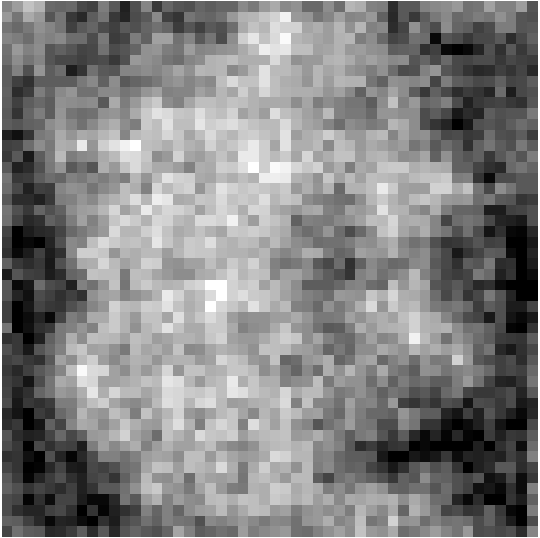
\includegraphics[scale=0.45]{reconstruction1_cropped}
		\caption{\small $P = 512$}
	\end{subfigure}%
	\begin{subfigure}[h]{0.45\textwidth}
		\centering
		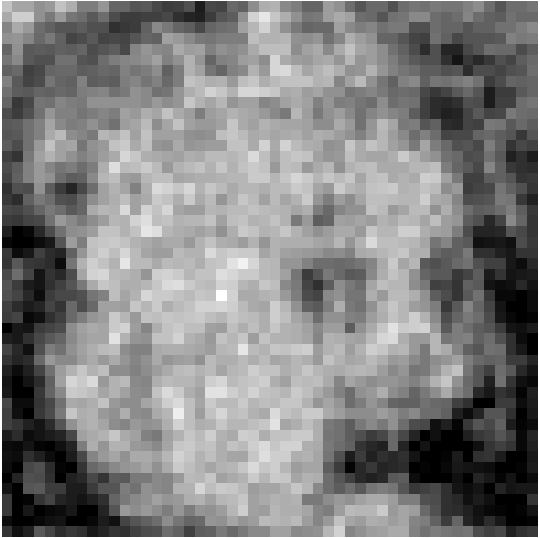
\includegraphics[scale=0.45]{reconstruction10_cropped}
		\caption{\small $P = 512\times 10$}
	\end{subfigure}%

		\begin{subfigure}[h]{0.45\textwidth}
		\centering
		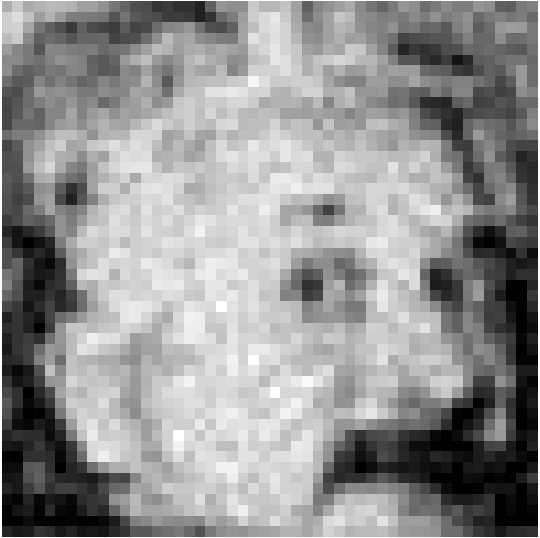
\includegraphics[scale=0.45]{reconstruction100_cropped}
		\caption{ \small $P = 512\times 10^2$ }
	\end{subfigure}%
	\begin{subfigure}[h]{0.45\textwidth}
		\centering
		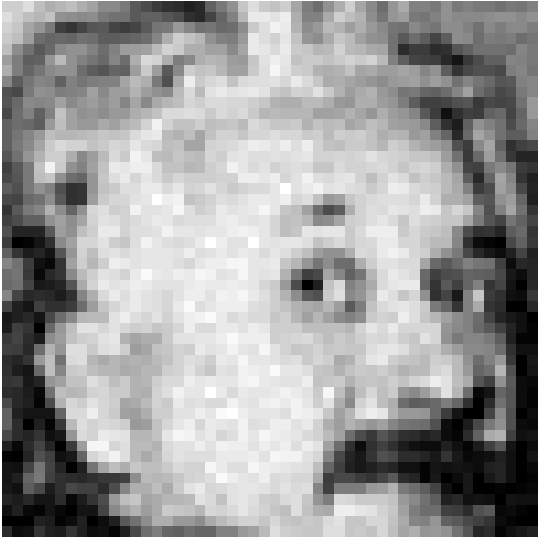
\includegraphics[scale=0.45]{reconstruction1000_cropped}
		\caption{\small $P = 512\times 10^3$}
	\end{subfigure}%


\end{figure}



\begin{figure}[h]
\centering
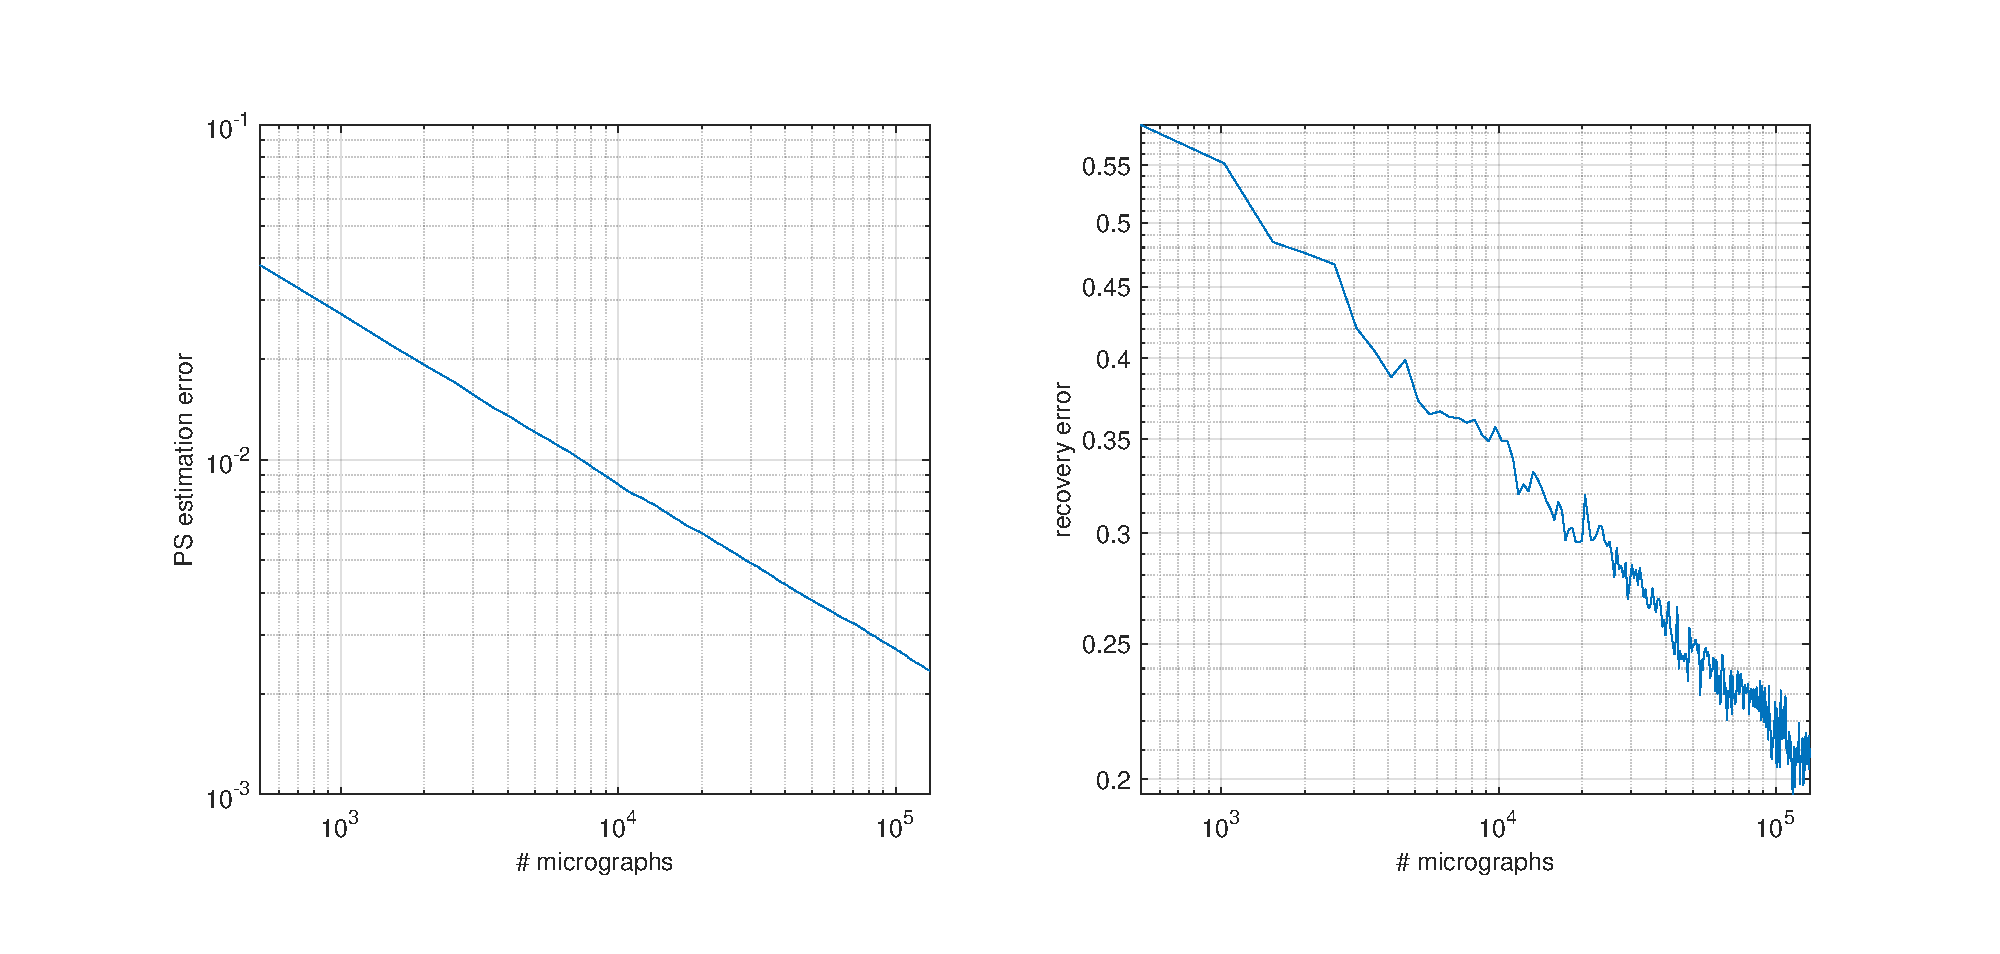
\includegraphics[scale=.7]{Einstein_progress}
\caption{\label{fig:error_per_micro} Relative root mean square error of the estimate of Einstein's image as a function of the number of observed micrographs (logarithmic scale along both axes.)}
\end{figure}




In the second experiment, three 1-D signals, each of length $L = 21$, appear at random locations in one long 1-D signal, which we call a micrograph by analogy. Any two occurrences are separated by at least 20 entries. The signals appear respectively about 30, 20 and 10 million times in a micrograph of length 12.3 billion. The micrograph is then contaminated with additive white Gaussian noise. This results in an $\SNR$ of about $1/9$, while about 10\% of the micrograph contains signal. Neither the number of occurrences nor the noise level $\sigma$ are known to the algorithm.

In the Methods section, we detail how autocorrelations of the micrograph can be used to estimate weighted averages of the autocorrelations of the target signals. The individual signals and their relative densities are then estimated from autocorrelations up to order three by solving a nonlinear least-squares problem.

Figure~\ref{fig:1Dheterosignals} shows how the estimates improve as we see a larger and larger fraction of the micrograph (that is, as more and more data becomes available.) As is clear from the picture, despite the high noise level which would make it very challenging to locate the individual signal occurrences, the signals can be estimated accurately given enough data. Furthermore, the \TODO{propensity\footnote{Might not be the right word; 'density' is not good because it might refer to the density of the particle for example, whereas here we mean to say the 'fraction of occurrences that come from a particular class'}} of each signal can also be estimated.



\begin{figure}[t]
	\centering
	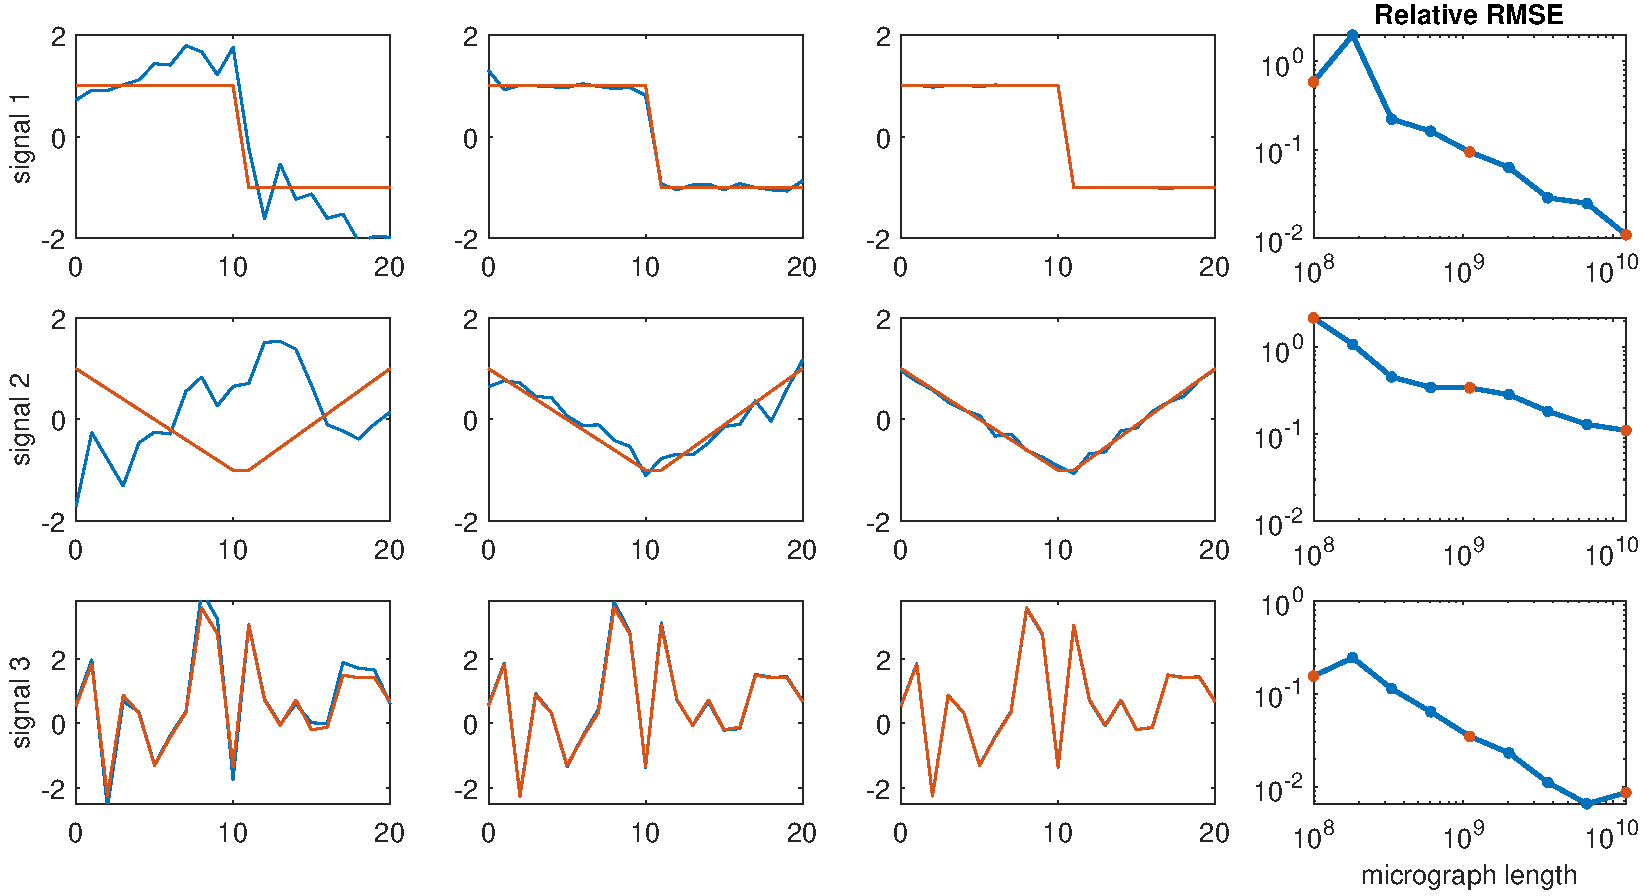
\includegraphics[width=\linewidth]{heterogeneous_progressive_n12300000000_466300}
	\caption{For the second experiment, each row shows, three times, one of the target signals (red), overlaid with an estimate (blue) obtained from a growing portion of the noisy micrograph (about $10^8$, $10^9$ and $10^{10}$ entries available to compute autocorrelations). The last column depicts evolution of the relative root mean square error in estimating each individual target signal. Signals 1 to 3 appear respectively about 30.0, 20.0 and 10.0 million times. With the whole micrograph available, the algorithm estimated those to be 29.8, 21.9 and 10.0 million, respectively.
	}
	\label{fig:1Dheterosignals}
\end{figure}


\TODO{The following was copying from the Methods section}


\paragraph{Numerical experiment with three 1-D signals.}


For the 1-D experiment depicted in Figure~\ref{fig:1Dheterosignals}, we fix $K = 3$ signals of length $L = 21$. Following the forward model described at the beginning of this section, we generate an observation $y$ of length $12.3 \cdot 10^9$. Each of the three signals appears, respectively (and approximately), $30.0 \cdot 10^6$, $20.0 \cdot 10^6$ and $10.0 \cdot 10^6$ times in $y$ for a total of exactly $60 \cdot 10^6$ occurrences, such that at least $L-1$ zeros separate any two occurrences of any signals. 
This is done by randomly selecting $60 \cdot 10^6$ placements in $y$, one at a time with an accept/reject rule based on the separation constraint and locations picked so far. For each placement, one of the three signals is picked at random according to the proportions $1/2, 1/3, 1/6$. Then, i.i.d.\ Gaussian noise with mean zero and standard deviation $\sigma = 3$ is added, to form the observed $y$. The resulting $\SNR$ of $y$
% sqrt((m_want*sum(X.^2)')/(sigma^2*n))
is about 1/9.


This is enough noise to make cross-correlations of $y$ even with the true signals display peaks at essentially random locations, uninformative of the actual locations of the signal occurrences. Thus, we contend that it would be difficult for any algorithm to locate the signal occurrences, let alone to classify them according to which signal appears where.

%\TODO{TB: I would place the equation counting argument in the theory section in the paragraph of open questions (I marked th place)}
%
Given the observation $y$, we proceed to compute the autocorrelations. The first-order autocorrelation is straightforward. For second-order autocorrelations, notice from equation~\eqref{eq:data_ac} that $a_y^2[\ell]$ suffers no noise-induced bias for $\ell$ in $1$ to $L-1$. Thus, we omit $\ell = 0$, which has the practical effect that we need not know $\sigma$ to make sense of the computed quantities. Likewise, for third-order autocorrelations, $a_y^3[\ell_1, \ell_2]$ for $0 \leq \ell_1, \ell_2 \leq L-1$ such that $\ell_2 \leq \ell_1$ includes all relevant entries for our purpose (this accounts for symmetries), and we further exclude any such that $\ell_1, \ell_2$ or $\ell_1 - \ell_2$ are zero to avoid the need to estimate $\sigma$---there are $\frac{(L-1)(L-2)}{2}$ remaining entries. We have
\begin{align*}
1 + (L-1) + \frac{(L-1)(L-2)}{2} = \frac{1}{2} L (L-1) + 1
\end{align*}
coefficients in total. Since we aim to estimate $KL$ parameters (for the $K$ signals of length $L$) plus $K$ parameters (for the densities $\gamma_k$), an absolute upper bound on $K$ (simply to ensure we have at least as many equations as we have unknowns) is
\begin{align*}
K(L+1) \leq \frac{1}{2} L (L-1) + 1.
\end{align*}
Thus, $(L-1)/2$ (up to a small approximation) is an absolute upper limit on $K$. \TODO{We may want to cite MRA literature here.}

In practice, the autocorrelations are computed on disjoint segments of $y$ of length $100\cdot10^6$ and added up, without correction for the junction points. Segments are handled sequentially on a GPU, as GPUs are particularly well suited to execute simple instructions across large vectors of data. If multiple GPUs are available, segments can of course be handled in parallel.

Having computed the moments of interest, we now estimate signals $x_1, \ldots, x_K$ and coefficients $\gamma_1, \ldots, \gamma_K$ which agree with the data. We choose to do so by running an optimization algorithm on the following nonlinear least-squares problem:
\begin{multline}
\min_{\substack{\hat x_1, \ldots, \hat x_K \in \reals^{W} \\ \hat \gamma_1, \ldots, \hat \gamma_K > 0}} w_1 \left( a_y^1 - \sum_{k=1}^K \hat \gamma_k a_{\hat x_k}^1 \right)^2 + w_2 \sum_{\ell = 1}^{L-1} \left( a_y^2[\ell] - \sum_{k=1}^K \hat \gamma_k a_{\hat x_k}^2[\ell] \right)^2 + \\ w_3 \sum_{\substack{2\leq\ell_1\leq L-1 \\ 1 \leq \ell_2 \leq \ell_1-1}} \left( a_y^3[\ell_1, \ell_2] - \sum_{k=1}^K \hat \gamma_k a_{\hat x_k}^3[\ell_1,\ell_2] \right)^2,
\label{eq:optim1D}
\end{multline}
where $W \geq L$ is the length of the sought signals and the weights are set to $w_1 = 1/2, w_2 = 1/2n_2, w_3 = 1/2n_3$, where $n_2, n_3$ are the number of moments used: $n_2 = L-1$, $n_3 = \frac{(L-1)(L-2)}{2}$ (weights could also be set in accordance with variance estimates as in~\cite{boumal2017heterogeneous}).

Setting $W = L$ (as is a priori desired) is problematic because the above optimization problems appears to have numerous poor local optimizers.
Thus, we first run the optimization with $W = 2L-1$. This problem appears to have few poor local optima, perhaps because the additional degrees of freedom allow for more escape directions. Since we hope the signals estimated this way correspond to the true signals zero-padded to length $W$, we extract from each one a subsignal of length $L$ that has largest $\ell_2$-norm. This estimator is then used as initial iterate for~\eqref{eq:optim1D}, this time with $W = L$. We find that this procedure is reliable for a wide range of experimental parameters. To solve~\eqref{eq:optim1D}, we run the trust-region method implemented in Manopt~\cite{manopt}, which allows to treat the positivity constraints on coefficients $\hat \gamma_k$. Notice that the cost function is a polynomial in the variables, so that it is straightforward to compute it and its derivatives.



\paragraph{Numerical experiment with 2-D image.}

For the 2-D experiment shown in Figures~\ref{fig:Einst_example} and~\ref{fig:error_per_micro}, we generate $P$ micrographs of size $4096\times 4096$ pixels. 
In each micrograph, we place Einstein's image (of zero mean) of size $50\times 50$  in random locations, while preserving the separation condition~\eqref{eq:spacing}.  
This is done by randomly selecting $4000$ placements in the micrograph, one at a time with
an accept/reject rule based on the separation constraint and locations picked so far.
On average, $700$ images are placed in each micrograph.   
Then, i.i.d.\ Gaussian noise with standard deviation $\sigma=3$ is added, inducing an $\SNR$ of approximately $1/20$.
An example of a micrograph's excerpt is presented in the right panel of Figure~\ref{fig:micro_example}.
%Different micrographs are handled sequentially on a GPU, as GPUs are particularly well suited to execute simple instructions across large vectors of data. If multiple GPUs are available, segments can of course be handled in parallel.


In this experiment, we assume we know the noise level $\sigma$ and the total number of occurrences of the target image across all micrographs.
In stark contrast with the 1-D setup, the second-order autocorrelation determines almost any target image uniquely, up to reflection through the origin~\cite{hayes1982reconstruction} (see also~\cite{bendory2017fourier} for a review). This is because the second-order autocorrelations correspond to the Fourier magnitudes of the signal through the 2-D Fourier transform. 
Therefore, we estimate the signal's Fourier magnitudes (or power spectrum) from the Fourier magnitudes of the micrographs, at the cost of one 2-D fast Fourier transform (FFT) per micrograph. These can be computed highly efficiently and in parallel.

To recover the target image from the estimated power spectrum, we use a standard phase retrieval algorithm called relaxed-reflect-reflect (RRR). This algorithm iterates the map
\begin{align*}
z & \leftarrow z + \beta (P_2(2P_1(z) - z) - P_1(z))
\end{align*}
on an image $z$ of size $2L\times 2L$.
We set the parameter $\beta$ to 1.
The map is designed so that, if the estimated power spectrum is exact, then fixed points contain Einstein's image in the upper-left corner of size $L \times L$, possibly reflected through its origin, and zeros elsewhere. The operator $P_2(z)$ combines the Fourier phases of  the current estimation $z$ with the estimated Fourier magnitudes. The operator $P_1(z)$ zeros out all entries of $z$ outside the $L\times L$ upper-left corner. 

In order to compare the performance in multiple cases and at different noise levels, the algorithm is stopped after a fixed number of iterations (1000) and the iterate with the smallest error compared to the ground truth (up to the reflection ambiguity) is chosen as the solution. While this cannot be done in practice (since we do not have access to the ground truth to determine which iterate is best), this procedure enables us to compare a large number of instances in different noise environments. \TODO{Note the last two sentences!}

\section{Application to cryo-EM}
\TODO{should be concise; the details are in the Nature paper}

\section{Discussion}

In the simplified model we examined, the aim is to estimate one, or possibly several, images from micrographs. Our strategy is to compute autocorrelation functions of the data and to relate these statistics to the unknown parameters. Recovering the parameters from the statistics reduces to solving a set of polynomial equations. Depending on the scenario, we did so using either a phase retrieval algorithm or a nonlinear least-squares algorithm.

The same general approach can, in principle, be applied directly to SPR from cryo-EM. Here, the micrographs contain numerous tomographic projections of molecules (possibly in different conformations) taken from unknown viewing directions. The aim is to estimate the 3-D volumes of the different conformations directly from micrographs. Each volume can be expanded linearly in a basis, so that the volume is characterized by its expansion coefficients. Since tomographic projection is a linear operation, autocorrelations of the micrographs (which can be estimated easily) are polynomial functions of the sought coefficients. Thus, autocorrelations of the micrographs provide a system of polynomial equations in the volume parameters, and the question becomes: are these equations sufficient to uniquely identify the volumes, and can we solve the system?

We show in Appendix~\ref{sec:cryoem} that the number of polynomial equations provided by the third-order autocorrelations is of the same order as the number of coefficients required to describe one volume \TODO{at resolution comparable to that of the particle projections---remove?}. This hints that it may be possible to reconstruct one or even several distinct volumes from these equations directly. Additional parameters in these equations could encode an unknown viewing direction distribution and an unknown conformation distribution, which could then also be estimated. Crucially, the outlined approach involves no particle picking, hence a fortiori no viewing direction estimation or conformation clustering. As a result, it may not be limited to large molecules in the same way that particle picking approaches are. Concerns for model bias would also greatly be reduced.


%While the field is currently dominated by Bayesian methods such as EM, they are intractable for such problems. As an alternative, we propose to use autocorrelation analysis technique that shares some common lines (did you get the wordplay?)  with Kam's method for ab initio modeling~\cite{kam1980reconstruction,levin20173d,singer2018mathematics}. That being said, the SPR model is far more complicated than the model presented here. In a future research, we hope to bridge this gap.

Of course, we recognize that significant challenges lay ahead for the implementation of the proposed approach to 3-D reconstruction directly from the micrographs. We discuss a few now.

One possible concern is that the numerical experiments conducted here suggest a large amount of data may be necessary.\footnote{Whether or not this large amount of data would be necessary for any method to succeed given the unfavorable $\SNR$ is an interesting research question.} Recent trends in high-throughput cryo-EM technology \TODO{?} give hope that this may be a lesser concern in the long term. Still, large amounts of data also imply large amounts of computations. On this front, we note that computing autocorrelations of low orders can be done efficiently on CPUs and GPUs, and in parallel across micrographs. It can even be done in streaming mode, as only one look at each micrograph is necessary. The output of this data processing stage is a succinct summary in the form of autocorrelation estimates: its size is a function of the resolution, not a function of the number of observed micrographs. Subsequent steps, which involve solving the system of polynomial equations, scale only in the size of that summary. Of course, an important question then is whether the equations can be solved meaningfully in practice. The proof-of-concept experiments above suggest they might.


Beyond data acquisition and computational challenges, there are modeling issues to consider.
As stated, our approach relies on two core assumptions that are not necessarily verified in SPR experiments.
First, we assume an additive white noise model, while in practice the noise may be structured or signal dependent. To address this point, it may be necessary to investigate better noise models and to extend the autocorrelation analysis accordingly.
Second, we assume that any two signal occurrences are sufficiently separated, and we use this assumption to derive algebraic relations between autocorrelations of the micrographs and autocorrelations of the target signals. 
Perhaps this separation could be induced by careful experimental design \TODO{?}.
Alternatively, if the signals are not well separated, one can introduce new parameters which encode the distribution of the spacing between occurrences. Here as well, relations between autocorrelation functions of the data and of the signals can be derived.

\TODO{Should we discuss CTF? Where, and to what extent?}

\TODO{Where and how do we cite Kam? Fred?}



\paragraph{Open theoretical questions.}

Our method of estimating $x$ uses the third-order moments of the observations. These empirical moments are used to obtain consistent estimators of population parameters related to the the mean and second- and third-order autocorrelations of $x$, to which we fit the signal $x$. Consequently, the number of signal occurrences $M$ should grow at least as fast as $1/\SNR^3$ to achieve a constant estimation error in the low $\SNR$ regime. In the related problem of multireference alignment~\cite{perry2017sample,abbe2017multireference}, this is optimal in the low $\SNR$ regime; we conjecture that the same is true for our problem.



Another interesting question is how many signals $x_1,\dots,x_K$ can be demixed from their mixed autocorrelation functions. In~\cite{boumal2017heterogeneous}, it was empirically observed that $K \sim \sqrt{L}$ signals can be estimated simultaneously from their mixed second- and third-order autocorrelations, using the least-squares procedure. In~\cite{weinthesis} [TKTK: add reference to Alex Wein's thesis, or put personal correspondence], this result is shown theoretically for a different, and much less efficient, algorithm. In our current setting, the additional parameters $\gamma$ and $\sigma$ make the problem more challenging; however, we conjecture that the number of estimable signals still grows like $\sqrt{L}$.

%%%That being said, we conjecture that the number of signals that can be demixed by an efficient algorithm is significantly smaller, and scales like $\sqrt{L}$; see~\cite{boumal2017heterogeneous,weinthesis} [TKTK: reference for missing Wein's thesis].

%The first entry $p[1]$ will represent the probability that two consecutive signals are separated by only one entry, $p[2]$ the probability for spacing of two entries and so on. Using this auxiliary variable $p$, one can write explicitly the relation between the autocorrelation functions of the data and those of the signal in a similar way to~\eqref{eq:data_ac}. 
%An interesting question is  under what conditions on $p$ and the signals, one can estimate the signals from the data.


\bibliographystyle{plain}
\bibliography{ref}



\appendix

\section{Proof of \eqref{eq:data_ac}} \label{sec:autocorrelation_computation}

Throughout the proof, we consider the case of one signal $K=1$. The extension to $K>1$ is straightforward by averaging the contributions of all signal with  appropriate weights; see~\cite{boumal2017heterogeneous}. 

We will let the number of instances of the signal $M$ grow with $N$, and write $M=M_N$ to emphasize this. We assume $M_N$ grows proportionally with $N$, and define:
%
\begin{equation}
\gamma = \lim_{N\to\infty} \frac{M_NL}{N}<1.
\end{equation}
%
We will assume that $M_N=\Omega(N)$, so that $\gamma>0$. In the sequel, we will suppress the explicit dependence of $M$ on $N$ for notational convenience.

We start by considering the mean of the data:
%
\begin{equation}
a_y^1 = \frac{1}{N}\sum_{i=0}^{N-1} y[i] =
\frac{1}{N/L}\sum_{j=0}^{M-1}\frac{1}{L}\sum_{i=0}^{L-1}x[i] +    
\underbrace{\frac{1}{N}\sum_{i=0}^{N-1}\varepsilon[i]}_{\text{noise term}}
\xrightarrow{a.s.}\gamma a_x^1,
\end{equation}
%
where the noise term converges to zero almost surely (a.s.) by the strong law of large numbers.

We proceed with the (second-order) autocorrelation for fixed $\ell\in[0,\ldots,L-1]$. We can compute:
%

\begin{align}
%
a_y^2[\ell] & = \frac{1}{N}\sum_{i=0}^{N-1-\ell}y[i]y[i+\ell]
\nonumber \\
& = \underbrace{\frac{1}{N}\sum_{j=1}^{M}\sum_{i=0}^{L-\ell-1}x[i]x[i+\ell]}_{\text{signal term}} + \underbrace{\frac{1}{N}\sum_{i=0}^{N-1-\ell}\varepsilon[i]\varepsilon[i+\ell]}_{\text{noise term}}
+ \underbrace{\frac{\TODO{1,2?}}{N} \sum_{j=1}^{M} \sum_{i=0}^{L-1} x[i] \varepsilon[s_j + i + \ell]}_{\text{cross-term}}.
%
\end{align}

The cross-terms are linear in the noise, and are easily shown to vanish almost surely in the limit $N\to\infty$, by the strong law of large numbers. As for the signal term, we break it into $M$ different sums, each containing one copy of the signal. This gives:
%
\begin{equation} \label{eq:2nd_moment_signal_term}
%
\frac{1}{N}\sum_{j=1}^{M}\sum_{i=0}^{L-\ell-1}x[i]x[i+\ell] = \frac{ML}{N}\frac{1}{L}\sum_{i=0}^{L-\ell-1}x[i]x[i+\ell]\xrightarrow{N\to\infty}\gamma a_x^2[\ell].
%
\end{equation}
%

We next analyze the pure noise term. When $\ell\neq 0$, we can break the noise term into a sum of independent terms:
%
\begin{equation}
%
\frac{1}{N}\sum_{i=0}^{N-1-\ell} \varepsilon[i]\varepsilon[i+\ell] = \frac{1}{\ell}\sum_{i=0}^{\ell-1}\frac{1}{N/\ell}\sum_{j=0}^{N/\ell -1} \varepsilon[j\ell + i] \varepsilon[(j+1)\ell + i].
%
\end{equation}
%
Each sum $\frac{1}{N/\ell}\sum_{j=0}^{N/\ell -1} \varepsilon[j\ell + i] \varepsilon[(j+1)\ell + i]$ is an average of $N/\ell$ independent terms with expectation zero, and thus converges to zero almost surely as $N\to\infty$. If $\ell=0$, then we have:
%
\begin{equation}
%
\frac{1}{N}\sum_{i=0}^{N-1} \varepsilon^2[i] \xrightarrow{a.s.} \sigma^2.
%
\end{equation}

We now analyze the third-order autocorrelation. Let us fix $\ell_1\geq\ell_2\ge0$. We have:
%
\begin{align}
%
&a_y^3[\ell_1,\ell_2] 
= \frac{1}{N}\sum_{i=0}^{N-1-\ell_1} y[i]y[i+\ell_1]y[i+\ell_2]
\nonumber \\
%
=& \underbrace{ \frac{ML}{N}\frac{1}{M}\sum_{j=1}^M 
	\frac{1}{L}\sum_{i=0}^{L-1-\ell_1}x[i]x[i+\ell_1]x[i+\ell_2]   }_{(1)}
+ \underbrace{\frac{1}{N}\sum_{i=0}^{N-1-\ell_1} \ep[i]\ep[i+\ell_1]\ep[i+\ell_2]}_{(2)}
\nonumber \\
&+ \underbrace{\frac{1}{N}\sum_{j=1}^{M} 
	\sum_{i=0}^{L-1} x[i]\ep[s_j + i+\ell_1]\ep[s_j+ i+\ell_2]}_{(3)}
+ \underbrace{\frac{1}{N}\sum_{j=1}^{M} 
	\sum_{i=0}^{L-1} \ep[s_j+i-\ell_1]x[i]\ep[s_j+ i+\ell_2-\ell_1]}_{(4)}
\nonumber \\
&+ \underbrace{\frac{1}{N}\sum_{j=1}^{M} 
	\sum_{i=0}^{L-1} \ep[s_j+i-\ell_2]\ep[s_j+i+\ell_1-\ell_2]x[i]}_{(5)}
+ \underbrace{\frac{1}{N}\sum_{j=1}^{M} 
	\sum_{i=0}^{L-\ell_1+\ell_2-1} \ep[s_j+i]x[i+\ell_1-\ell_2]x[i]}_{(6)}
\nonumber \\
&+ \underbrace{\frac{1}{N}\sum_{j=1}^{M} 
	\sum_{i=0}^{L-\ell_2-1} x[i]\ep[s_j + i+\ell_1]x[s_j+ i+\ell_2]}_{(7)}
+ \underbrace{\frac{1}{N}\sum_{j=1}^{M} 
	\sum_{i=0}^{L-\ell_1-1} x[i]x[i+\ell_1]\ep[s_j+ i+\ell_2]}_{(8)}.
%
\end{align}
%
Terms (6), (7) and (8) are linear in $\ep$, and can easily be shown to converge to 0 almost surely by the law of large numbers, by similar arguments as used previously. Term (1) converges to $\gamma a_x^3[\ell_1,\ell_2]$ almost surely, for the same reasons as~\eqref{eq:2nd_moment_signal_term}. To deal with terms (2)--(5), we must distinguish between different values of $\ell_1$ and $\ell_2$.

{\bf Case 1:} $0 < \ell_2 < \ell_1$. Here, all summands with elements of $\ep$ involve products of distinct entries, which have expected value 0. Consequently, the usual argument shows that terms (2)--(5) all converge to 0 almost surely as $N \to \infty$.

{\bf Case 2:} $0=\ell_2 < \ell_1$. Term (2) is an average of products of the form $\ep[i]^2\ep[i+\ell_1]$, which have mean zero; consequently, term (2) converges to 0 almost surely. The same argument as for Case 1 shows that (3) and (5) also converge to 0. For term (4), we write:
%
\begin{align}
%
&\frac{1}{N}\sum_{j=1}^{M} 
\sum_{i=0}^{L-1} \ep[s_j+i-\ell_1]x[i]\ep[s_j+ i+\ell_2-\ell_1]
\nonumber \\
&= \frac{ML}{N}\frac{1}{L}\sum_{i=0}^{L-1}x[i] \frac{1}{M}\sum_{j=1}^{M} \ep[s_j+i-\ell_1]^2
\xrightarrow{N\to\infty} \gamma \frac{1}{L} \sum_{i=0}^{L-1}x[i] \sigma^2 = \gamma a_x^1 \sigma^2.
%
\end{align}

{\bf Case 3:} $0<\ell_2 = \ell_1$. An argument nearly identical to that for Case 2 shows that terms (2), (4) and (5) converge to 0, while term (3) converges to $\gamma a_x^1 \sigma^2$.

{\bf Case 4:} $0=\ell_2 = \ell_1$. The same argument as for term (4) in Case 2 shows that terms (3), (4) and (5) all converge to $\gamma a_x^1 \sigma^2$. Term (2) is an average of $\ep[i]^3$, which is mean zero; consequently, it converges to 0.


This completes the proof of \eqref{eq:data_ac}.








%%% We conjecture that similarly to the 


%%%In methods which are based on detection and averaging, the number of signals occurrences  must scale like $1/\SNR$. 

\begin{comment}

Another interesting question is how many signals $x_1,\dots,x_K$ can be demixed from their mixed autocorrelation functions. For second-order moments, notice from equation~\eqref{eq:data_ac} that $a_y^2[\ell]$ suffers no bias for $\ell$ in $1$ to $L-1$. Thus, we omit $\ell = 0$, which has the practical effect that we need not know $\sigma$ to estimate the moments. Likewise, for third-order moments, $a_y^3[\ell_1, \ell_2]$ for $0 \leq \ell_1, \ell_2 \leq L-1$ such that $\ell_2 \leq \ell_1$ includes all relevant moments for our purpose, and we further exclude any such that $\ell_1, \ell_2$ or $\ell_1 - \ell_2$ are zero to avoid biased elements---there are $\frac{(L-1)(L-2)}{2}$ remaining moments. As a result, it is unnecessary to estimate $\sigma$. We have 
\begin{align*}
1 + (L-1) + \frac{(L-1)(L-2)}{2} = \frac{1}{2} L (L-1) + 1 \approx L/2,
\end{align*}
moments in total.

In the related problem of demixing signals from their periodic autocorrelation functions, there is evidence that the number of identifiable signals is equal to the number of different equations~\cite{bandeira2017estimation}. Based on this, we conjecture that the same phenomenon holds here as well, namely that $L/2$ signals are identifiable.  That being said, we conjecture that the number of signals that can be demixed by an efficient algorithm is significantly smaller, and scales like $\sqrt{L}$; see~\cite{boumal2017heterogeneous,weinthesis} [TKTK: reference for missing Wein's thesis].

\end{comment}


\section{Proof of Proposition~\ref{prop:gamma_sigma}} \label{sec:proof_prop_gamma_sigma}

We will prove that both $\sigma$ and $\gamma$ are identifiable from the observed first three moments of $y$. For convenience, we will work with $\beta = \gamma / L$ rather than $\gamma$ itself. We will construct two quadratic equations satisfied by $\beta$ from observed quantities, independent of $\sigma$. Then, we will show that these equations are independent, and hence that $\beta$ is uniquely defined.  Given $\beta$, we can estimate $\sigma$ using Proposition~\ref{prop:gamma}.

Throughout the proof, it is important to distinguish between observed and unobserved values. 
We denote the observed values by $E_i$ or $a_y^1,a_y^2,a_y^3$, while using $F_i$ for functions of the signal's autocorrelations. 

Recall that $a_y^1 = \beta(\one^Tx)$ and  
and $a_y^2[0] = \beta\|x\|^2+\sigma^2$, where $\one\in\RL$ stands for vector of ones. Taking the product:
\begin{equation}\label{eq:E1}
\begin{split}
E_1 &:= a_y^1a_y^2[0] =  (\beta(\one^Tx))(\beta\|x\|^2+\sigma^2) \\
& = \sigma^2a_y^1 + \beta^2F_1,
\end{split}
\end{equation}
where $F_1 := a_x^3[0,0] + \sum_{j=1}^{L-1}(a_x^3[j,j] + a_x^3[0,j])$. 
The terms of $F_1$ can be also estimated from $a_y^3$, while taking the scaling and bias terms into account:
\begin{equation} \label{eq:E2}
E_2:= \beta F_1 + (2L+1)\sigma^2a_y^1.
\end{equation}
Therefore, from~\eqref{eq:E1} and~\eqref{eq:E2} we get
\begin{equation} \label{eq:E12}
E_2\beta -(2L+1)\sigma^2\beta a_y^1 = E_1-\sigma^2a_y^1.
\end{equation}
Let $a_y^2:=\sum_{j=0}^{L-1}a_y^2[j]$ and recall from Proposition~\ref{prop:gamma}:
\begin{equation} \label{eq:sigma2}
\sigma^2 = a_y^2 - (a^1_y)^2/(\beta L). 
\end{equation} 
Plugging into~\eqref{eq:E12} and rearranging we get 
\begin{equation} \label{eq:quad1}
\mathcal{A}\beta^2 + \mathcal{B}\beta + \mathcal{C} = 0,
\end{equation}
where 
\begin{align*}
\mathcal{A} &= E_2 - (2L+1)a_y^1a_y^2, \\ 
\mathcal{B} &= -E_1 + \frac{2L+1}{L}(a_y^1)^3 + a_y^1a_y^2  , \\
\mathcal{C} &= -(a_y^1)^3/L.
\end{align*}
Importantly, these coefficients are observable quantities. 

We are now proceeding to derive the second quadratic equation. We notice that 
\begin{equation} \label{eq:E3}
E_3  = \frac{1}{L}(a_y^1)^3 = \frac{1}{L}\beta^3 (\one ^Tx)^3   = \frac{1}{L}\beta^3 F_2,
\end{equation}
where 
\begin{equation*}
F_2 =  a_x^3[0,0] + 3\sum_{j=1}^{L-1}a_x^3[j,j] + 3\sum_{j=1}^{L-1}a_x^3[0,j] + 6\sum_{1\leq i < j\leq L-1}a_x^3[i,j].
\end{equation*}
On the other hand, from $a_y^3$ we can directly estimate $F_2$ up to scale and bias
\begin{equation} \label{eq:E4}
E_4 = \beta F_2 + (6L-3)\sigma^2a_y^1.
\end{equation}
Taking the ratio:
\begin{equation*} 
\frac{E_4}{E_3} = \frac{L}{\beta^2} + \frac{(6L-3)L\sigma^2a_y^1}{E_3}, 
\end{equation*}
we conclude:
\begin{equation*}
\sigma^2 = \frac{E_4}{a_y^1L(6L-3)}  - \frac{E_3}{\beta^2a_y^1(6L-3)}.
\end{equation*}
Using~\eqref{eq:sigma2} and rearranging we get the second quadratic:
\begin{equation} \label{eq:quad2}
\mathcal{D}\beta^2 + \mathcal{E}\beta + \mathcal{F} = 0,
\end{equation}
where
\begin{align*}
\mathcal{D} &= a_y^2 - \frac{E_4}{a_y^1L(6L-3)}, \\ 
\mathcal{E} &= -(a_y^1)^2/L, \\
\mathcal{F} &= \frac{E_3}{a_y^1(6L-3)}.
\end{align*}

To complete the proof, we need to show that the two quadratic equations~\eqref{eq:quad1} and~\eqref{eq:quad2} are independent. To this end, it is enough to show that the ratio between the coefficients is not the same. 
From~\eqref{eq:quad1} and~\eqref{eq:E1}, we have 
\begin{equation*}
\begin{split}
\frac{\mathcal{B}}{\mathcal{C}} &= \frac{LE_1 - (2L+1)(a_y^1)^3 - La_y^1a_y^2}{(a_y^1)^3} \\&= \frac{La_y^2[0] - (2L+1)(a_y^1)^2 - La_y^2}{(a_y^1)^2}.
\end{split}
\end{equation*}
In addition, using~\eqref{eq:E3}
\begin{equation*}
\frac{\mathcal{E}}{\mathcal{F}} = \frac{(3-6L)(a_y^1)^3}{LE_3} = 3 - 6L . 
\end{equation*}

Now, suppose that the quadratics are dependent. Then, $\frac{\mathcal{B}}{\mathcal{C}} =\frac{\mathcal{E}}{\mathcal{F}} $, or, 	
\begin{equation*}
La_y^2[0] - (2L+1)(a_y^1)^2 - La_y^2 = (a_y^1)^2(3-6L)
\end{equation*}
Rearranging the equation and writing in terms of $x$ we get 
\begin{equation} \label{eq:cond}
4(L-1)\beta (a_x^1)^2  - \sum_{i=1}^{L-1} a_x^2[i] = 0.
\end{equation}	
For generic $x$,  this polynomial equation is not satisfied. Therefore,  the equations are independent. 
More than that, for any nonzero $x$, $(a_x^1)^2 >\sum_{i=1}^{L-1} a_x^2[i]$. Therefore, if $4(L-1)\beta \geq 1$, or,
\begin{equation*}
\beta \geq \frac{1}{4(L-1)},
\end{equation*}
the condition~\eqref{eq:cond} cannot be satisfied for any signal. 


\end{document}

